\section{Descrizione Dataset}
Il dataset è composto da 373 record organizzati in 15 colonne, ognuna delle quali esplicita un attributo della tupla. Di seguito la loro descrizione:
\begin{itemize}
\setlength\itemsep{0.2em}
    \item Subject ID: sequenza di caratteri alfanumerici che identifica il paziente
    \item MRI ID: numero identificativo della risonanza magnetica eseguita sul paziente. Compare come il Subject ID seguito dal numero della risonanza magnetica
    \item Visit: numero della visita dell'individuo
    \item MR delay: tempo intercorso in secondi tra l'iniezione del liquido di contrasto e l'esecuzione della risonanza
    \item M/F: genere del paziente (maschio o femmina)
    \item Hand: mano dominante del soggetto (tutti i soggetti interessati usano la mano destra)
    \item Age: età del paziente
    \item EDUC: anni di istruzione
    \item SES: status socioeconomico assegnato dall'Hollingshead Index of Social Position sulla base di un punteggio che va da 1 (più alto status) a 5 (più basso status)
    \item MMSE: Mini-Mental State Examination, un test neuropsicologico costituito da 30 domande utilizzate per verificare lo stato cognitivo. Va da 1 (peggior stato) a 30 (miglior stato). Con un punteggio inferiore a 24 il paziente presenta indebolimento cognitivo ma non necessariamente demenza;
    \item eTIV: estimated Intracranical Volume, stima del volume intracranico in cm$^3$
    \item nWBV: normalized Whole-Brain Volume, espresso come percentuale del volume del cervello in rapporto con il volume intracranico (eTIV)
    \item ASF: Atlas Scaling Factor, determinante della matrice di trasformazione tra lo spazio della MRI e la mappa utilizzata per strutturare il cervello. In pratica restituisce il raporto fra la misura del volume dell'immagine e della mappa. 
    \item CDR: Clinical Dementia Rating, scala numerica che identifica la gravità della demenza. In particolare si ha 0 per un paziente normale, 0.5 per dubbia demenza, 1 per lieve demenza, 2 per moderata demenza, 3 per grave demenza. Infine 4 e 5 rappresentano i casi più gravi in assoluto.
    \end{itemize}

Nel nostro caso abbiamo la seguente distribuzione di CDR:    
\begin{figure}[H]
	\centering
	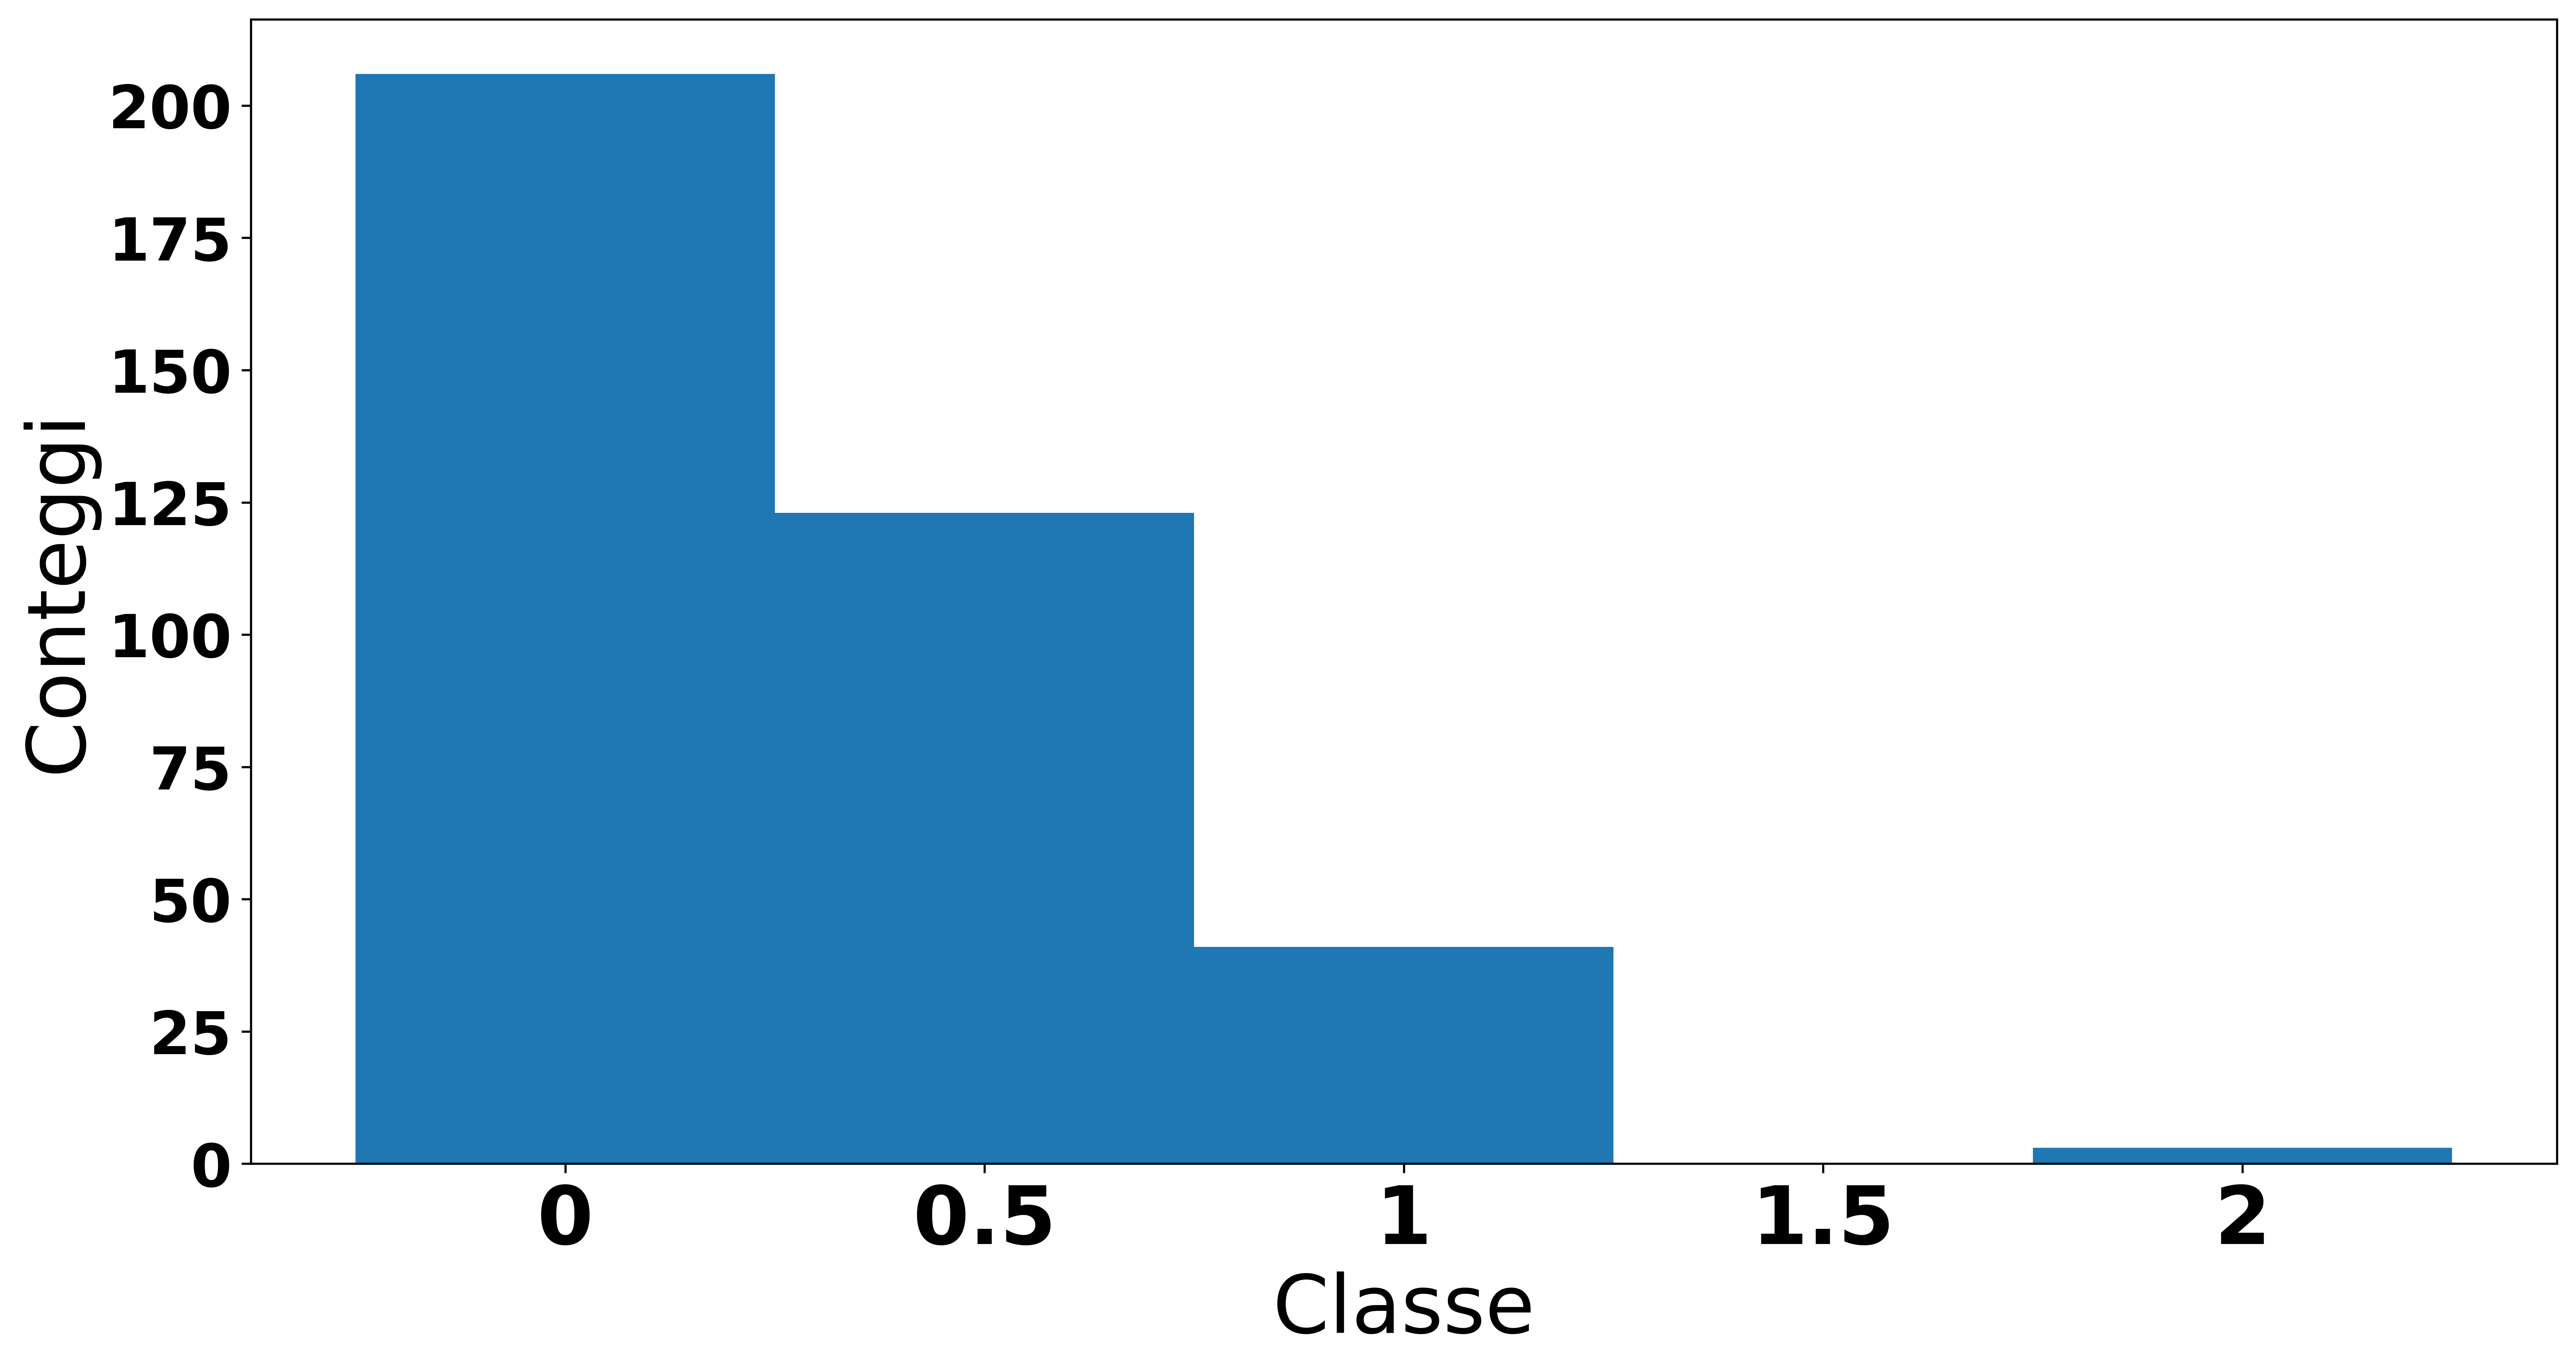
\includegraphics[height=0.55 \linewidth]{bar_plot.png}
	\caption{I valori più bassi sono molto più numerosi e non è presente la classe 1.5}
\end{figure}
    
    
    
    
    